% Name: Linear fit with confidence band
% Description: Data points, a fitted line, and a shaded band that widens away from the center of the data.
% Tags: regression, confidence band, fill between, fit

\usepackage{pgfplots}
\usepgfplotslibrary{fillbetween}
\pgfplotsset{compat=1.18}

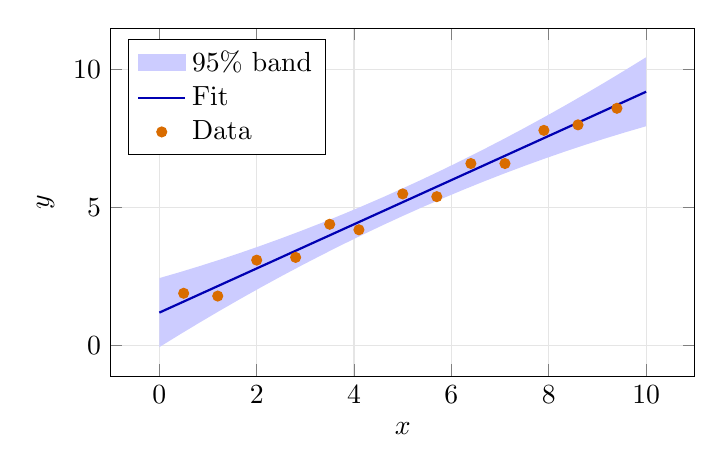
\begin{tikzpicture}
  \begin{axis}[
    width=9cm, height=6cm, xlabel=$x$, ylabel=$y$,
    legend pos=north west, legend cell align=left,
    grid=major, grid style={gray!20},
  ]
    \addplot[name path=upper, draw=none, domain=0:10, forget plot] {1.2 + 0.8*x + 0.5 + 0.03*(x - 5)^2};
    \addplot[name path=lower, draw=none, domain=0:10, forget plot] {1.2 + 0.8*x - 0.5 - 0.03*(x - 5)^2};
    \addplot[blue!20] fill between[of=upper and lower];
    \addplot[blue!70!black, thick, domain=0:10] {1.2 + 0.8*x};
    \addplot[only marks, mark=*, mark size=1.8pt, orange!85!black] coordinates {
      (0.5,1.9) (1.2,1.8) (2,3.1) (2.8,3.2) (3.5,4.4) (4.1,4.2) (5,5.5)
      (5.7,5.4) (6.4,6.6) (7.1,6.6) (7.9,7.8) (8.6,8.0) (9.4,8.6)
    };
    \legend{95\% band, Fit, Data}
  \end{axis}
\end{tikzpicture}
